\documentclass{school-22.101-notes}
\date{October 14, 2011}

\begin{document}
\maketitle

\lecture{Intro to Nuclear Structure}
Prof. Li on 10/10/12: in the classical view, particles have labels as in Fig.~\ref{classical-identity}. 

\begin{figure}[ht]
  \centering
  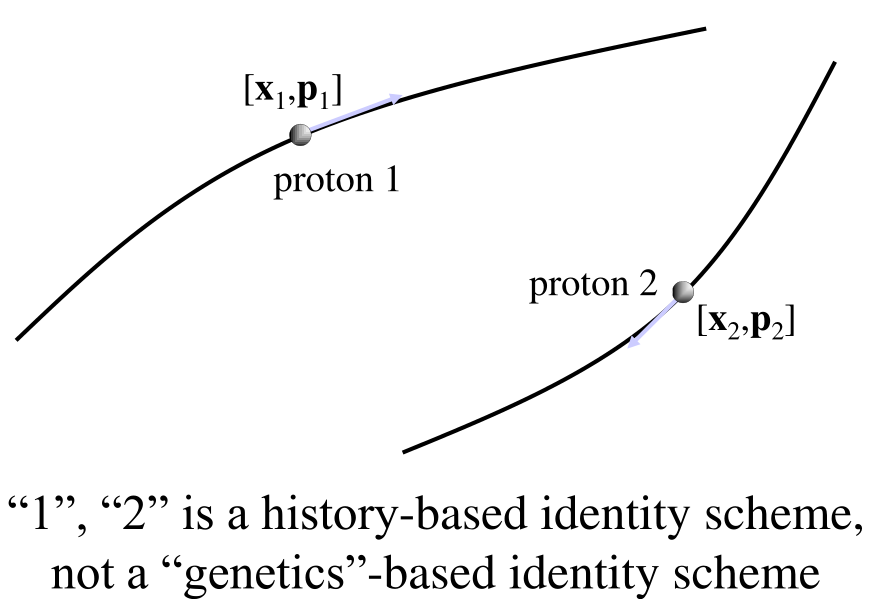
\includegraphics[width=3.5in]{images/ns/classical-identity.png}
  \caption{Classical Objects have Identities} \label{classical-identity}
\end{figure}

In the quantum view, we do not talk about the classical particles anymore; nothing is confined perfectly because there is no infintie potential in reality (that is, no hard spheres). 

Instead, we discuss wavepacks, that is, a distribution of nucleon charge and mass as in Fig.~\ref{quantum-identity}. Moreover, we separate a particle/wave's identity into two portions: the orbitals $X_1, X_2$, and the occupants $a,b$ label. For instance, if we measure at any time, we get $X_1, X_2$, but we do not know which particle/wave is which; we arbitrary assign $a,b$, and measure again and get $X_1, X_2$ again but again we do not know which one is $a$ which one is $b$ again. That is, \hi{two wavepacks have `distinguishable orbitals, indistinguishable occupants.'}

\begin{figure}[ht]
  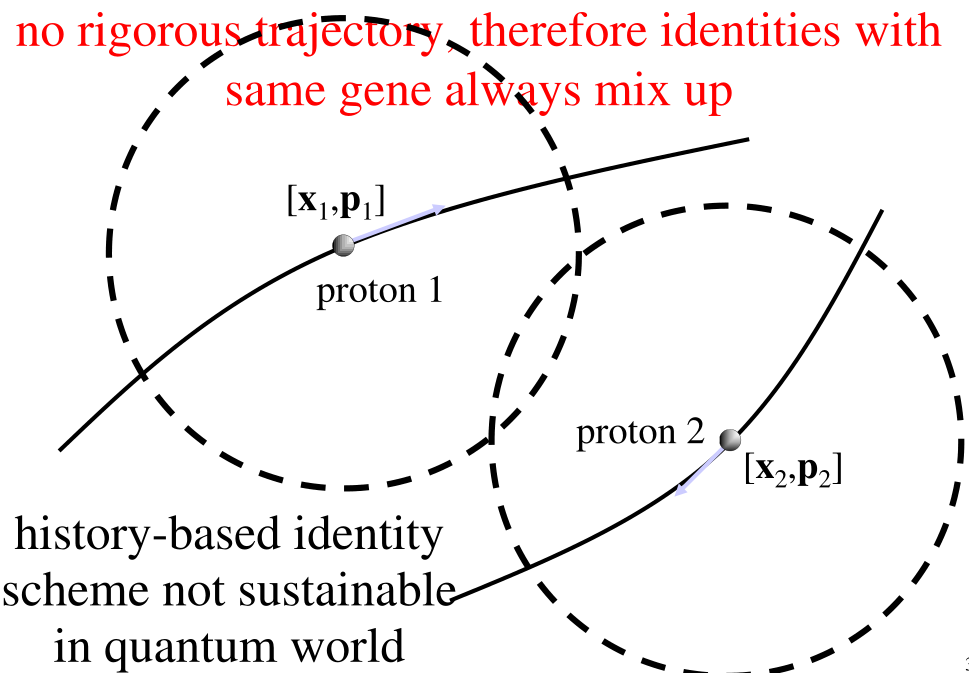
\includegraphics[width=3.2in]{images/ns/quantum-identity.png}
  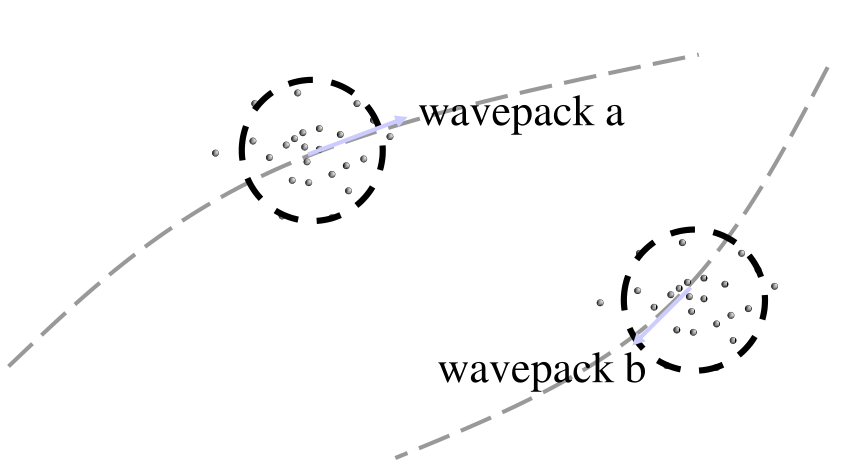
\includegraphics[width=3.2in]{images/ns/quantum-identity-2.png}
  \caption{Quantum Objects Are Wavepacks} \label{quantum-identity}
\end{figure}





We can measure three things: size, spin, and magnetic moment $\mu$. We will discuss each of the three measurements separately. 


\topic{Multi-Neutron Wavefunction}
We define single particle spin-orbital function $\phi(X)$. For instance, for a neutron $a$, its spin-orbital function is, 
\eqn{ \phi_a(X_1) = f(x_1) \ket{\up}_1 + g(x_1) \ket{\down}_1   }
\eqn{ \phi_a(X_2) = f(x_2) \ket{\up}_2 + g(x_2) \ket{\down}_2   }

For two neutrons (with the label $a,b$, though we do not know which one is correspond to $X_1$, which one correspond to $X_2$), 
\eqn{ \Psi(X_1, X_2) &= \left| \begin{array}{cc} 
    \phi_a (X_1) & \phi_b (X_1) \\
    \phi_a (X_2) & \phi_b (X_2) 
    \end{array} \right| = \phi_a(X_1) \phi_b (X_2) - \phi_b(X_1) \phi_a (X_2) }

Comments: 
\begin{itemize}
\item Notice the above formalism automatically satisfies the symmetry requirement. 
\item The fact that the $\Psi(X_1, X_2)$ depends on the product of two single-particle's wavefunction, that is, $\Psi(X_1, X_2)$ contains $\ket{\up}_1 \ket{\up}_2$ terms, implies that the total behavior is dependent on the interaction of the two particles. This leads to Quantum Entanglement. 
\end{itemize}

For three neutrons: 
\eqn{ \Psi(X_1, X_2, X_3)  = \det \left| 
\begin{array}{ccc} \phi_a (X_1) & \phi_b (X_1) & \phi_c (X_1) \\
  \phi_a (X_2) & \phi_b (X_2) & \phi_c (X_2) \\
  \phi_a (X_3) & \phi_b (X_3) & \phi_c (X_3) 
\end{array} \right| 
+ \det \left| 
\begin{array}{ccc} \phi_d (X_1) & \phi_e (X_1) & \phi_f (X_1) \\
  \phi_d (X_2) & \phi_e (X_2) & \phi_f (X_2) \\
  \phi_d (X_3) & \phi_e (X_3) & \phi_f (X_3) 
\end{array} \right|  + \cdots }


\topic{Nucleon Measurables}
Recall that in quantum world nucleon charge and mass are distributions. 

\begin{enumerate}
\item Nucleon Size: 
  \begin{itemize}
  \item One way to measure the nucleon `size' would be to measure the nucleon charge from high-energy electron scattering, then define the root mean squared nuclear radius from the nucleon charge distribution. 

  \item Alternatively people come up with the $A^{1/3}$ law: 
    \eqn{ R = R_0 A^{1/3} \approx 1.2 \fm A^{1/3} }
    which means that the density of nuclear charges inside a nuclide is a constant. 

  \item One can measure the nuclear mass distribution from Rutherford scattering, $\alpha$ decay, and pionic X rays. It turns out that the nuclear matter distribution closely matches that of the nuclear charges. That is, neutrons and protons form a nearly homogeneous mixture, and there is not much segregation on the nuclide surface. 
  \end{itemize}

\item Spin/Angular Momentum. The state of a nuclide (nuclide composite of nucleon) can be labled as $\boxed{I^{\Pi}}$, where $I$ is the total angular momentum of the nuclide, and $\Pi$ is the parity of the nuclide. 

To start, we consider labeling each nucleon (inside of the nuclide) by orbital angular momentum $l$, spin $s$, and total angular momentum $j$. With a central potential, even with self spin-orbit interactions, 
\eqn{ [\vec{l} \cdot \vec{s}, \vec{l}^2 ] = [ \vec{l} \cdot \vec{s}, \vec{s}^2] = 0 }
which implies that $l(l+1), s(s+1), j(j+1)$ are reasonable quantum numbers to use. 

If the nuclide is stationary, the total angular momentum would be, 
\eqn{ \vec{I} = \Sum_{i=1}^A \vec{j}_i }
Since we are talking about nucleons being neutrons and protons (whose spins are 1/2, and $l =$ integers), $\vec{j}_i$ can only be half integers, and follow that 
\eqn{ I = \left\{ \begin{array}{cc} \mbox{half integer} & \mbox{If A is odd} \\ \mbox{integer} & \mbox{If A is even}   \end{array} \right. }

Often times nucleons form pairs (the pair's angular momentum is zero) to minimize energy, and a single nucleon can determine $I = j$. For instance all the even-even nuclides have $I=0$, which is a strong evidence for the nuclear pairing force. 

\item Parity. By definition, a parity operator $\hat{P}$ satisfies (notice this is different from the permutation operator above), 
\eqn{ \hat{P} \left( \ket{\up} f(x,y,z) + \ket{\down} g(x,y,z) \right) = \ket{\up} f(-x, -y, -z) + \ket{\down} g(-x,-y,-z) }
That is, 
\eqn{ \hat{P} \phi(X) = \phi(X) (-1)^l }
Recap: $\hat{P}_{ij}$ commutes with the Hamiltonian, $[H, \hat{P}_{ij}] = 0$. 
\eqn{ \boxed{ \Pi = \Prod_{i=1}^A \Pi_i = (-1)^l}  }

\item Magnetic Momentum. Magnetic moment $\mu$ can be defined as, 
\eqn{ \vec{\mu} = I A \vec{n}}
where $A$ is the area, $I$ is the angular momentum, and $\vec{n}$ is the magnetic field direction. We can simplify the above expression to be, 
\eqn{ \vec{\mu} = q \frac{v}{2 \pi r} \pi r^2 = \frac{\hbar q (vrm)}{2m} = \frac{\hbar q}{2m} \frac{l}{\hbar} }

Example: for an electron and a proton, their magnetic moments are respectively
\eqn{ \mu_B  = \frac{e \hbar}{2m_e} = 5.78 \times 10^{-5} \eV/\mathrm{T} }
\eqn{ \mu_N = \frac{e \hbar}{2m_p} = 3.15 \times 10^{-8} \eV/\mathrm{T} }

That is, we can write the orbital contribution to magnetic moment: 
\eqn{ \vec{\mu}_{l_i} = \mu_N \frac{l_i}{\hbar} g_l(i)}
where $g_l (p) = 1, g_l (n) = 0, g_l (e^-) = -1$. 

Similarly the spin contribution to magnetic moment: 
\eqn{ \vec{\mu}_{s_i} = \mu_N \frac{S_i}{\hbar} g_s (i) }
where $g_s(p) = 5.59, g_s(n) = -3.83, g_s(e^-) = -2.00$. 

Together, the magnetic momentum of a composite can be written as, 
\eqn{ \boxed{ \vec{\mu} = \Sum_{i=1}^A \vec{\mu}_i =  \mu_N  \Sum_{i=1}^A \left( \frac{\vec{S}_i}{\hbar} g_s (i) + \frac{\vec{l}_i}{\hbar} g_l (i) \right)  } } 
\end{enumerate}

\end{document}
